\section*{Detalii despre dezvoltarea aplicației}
	Dezvoltarea aplicației a început cu prima întâlnire între fondatorii companiei, cei ce aveau grijă de sistemul de rapoarte în Excel și mine.
	Ne-am așezat la masă și astfel am început să discutăm despre cerințele aplicației.

	Accentul s-a pus pe dorința de a scoate rapoarte mai ușor, fără a putea interveni eroarea umană.
	Să nu se mai verifice manual câte asigurări s-au vândut într-o perioadă de timp determinată.
	Eliminarea nevoii de a căuta în fiecare fișier trimis săptămânal de Altex / Media Galaxy.

	Pe tot parcursul dezvoltării aplicației, am fost singurul ce s-a ocupat de aranjarea sistemului informatic, migrarea spre o soluție de găzduire partajată, construirea bazei de date, relațiilor, securitatea datelor și interacțiunii utilizatorului cu aplicația.

	Structura bazei de date a fost gândită prima oară a fi rigidă, a forța utilizatorul și persoanele ce se ocupă de gestiunea lor să introducă datele corecte, a nu avea probleme ulterioare.
	Ideea a fost întâmpinată cu rezistență, datorită libertății oferite de Excel, dar într-o scurtă perioadă de timp, rigiditatea a dat roade.
	Rapoartele erau exacte și erorile ne-existente.

	Interacțiunea cu utilizatorul de rând a fost gândită a fi cât mai rapidă.
	Atunci când intră pe pagina aplicației, el poate deja să completeze cererea de despăgubire, așa cum se poate observa în poza \ref{fig:pagina_principala}.
	Utilizatorul este îndrumat pentru a completa cât mai detaliat detaliile despre cererea de despăgubire și este avertizat atunci când apare o eroare sau a uitat să completeze un câmp necesar.
	\begin{figure}
	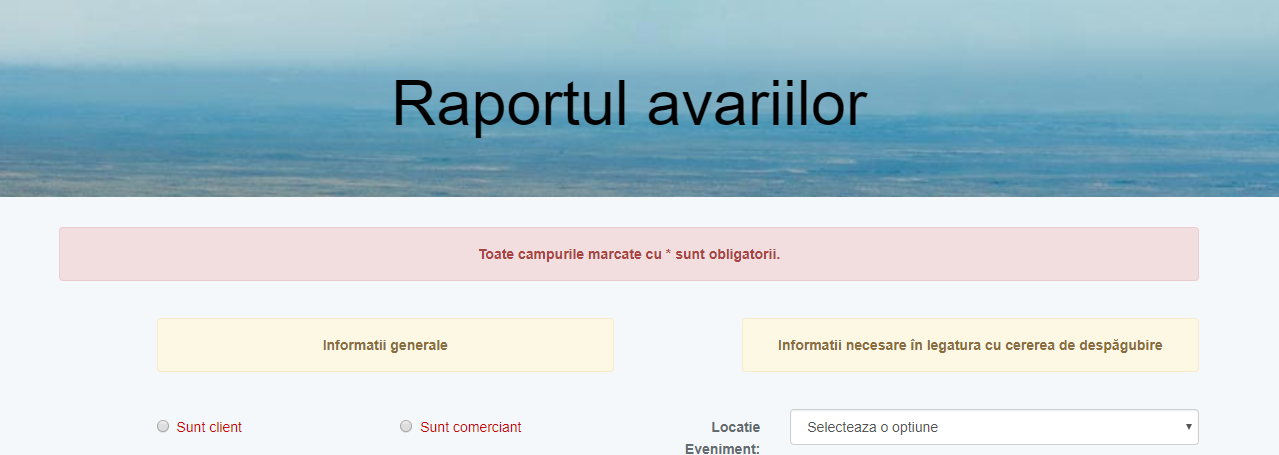
\includegraphics[width=\linewidth]{../imagini/main.png}
	\caption{Pagina principală a \url{https://fandu.info}}
	\label{fig:pagina_principala}
	\end{figure}

	Am ales să salvez toate datele utilizatorului în baza proprie de date, la o companie de încredere ce oferă soluții de găzduire partajată \url{https://xServers.ro}\cite{xservers}.
	Dar pozele și spațiul de stocare a pdf-urilor încărcate de utilizatori sunt găzduite de Amazon Web Services\cite{aws}, pentru a beneficia de prețul redus și valabilitatea extinsă a fișierelor pe „cloud”.

	Revenind la soluția de găzduire partajată, am ales xServers.ro\cite{xservers} pentru că aplicația se încadrează lejer în oferta lor.
	Cel mai important atu este traficul de internet necontorizat și spațiu de stocare suficient.

	Soluția de backup, oferită de cei ce găzduiesc aplicația, salvează baza de date în fiecare zi.

	De asemenea, mă ocup personal pentru a asigura un backup săptămânal a bazei de date pe un volum encriptat cu „VeraCrypt”\cite{veracrypt}, un utilitar gratuit ce construiește un disc virtual securizat într-un simplu fișier.

	Cele două soluții complementare asigură securitatea datelor și rezolvarea instantanee a problemelor bazei de date, cheia aplicației.

	Codul sursă este ținut într-un proiect „git”, un sistem de gestionare și versionare a codului de programare, încărcat pe GitHub, un aliat de încredere oricărui programator.
